\subsubsection{Módulo matemático en Osciloscopios Digitales}

    Con la llegada de los osciloscopios digitales con módulo matemático, estos mismos 
    fueron reemplazando los analizadores de fourier convencionales.
    Dicho módulo posee un algoritmo de transformada rápida de fourier (FFT), donde 
    a partir de las muestras tomadas en el dominio del tiempo de una señal de entrada,
    se realiza la conversion de la señal con la FFT al dominio de la frecuencia.
    El esquema en bloques simplificado se puede observar en la Figura~\ref{fig:MathModuleEnOscil}.
        \begin{figure}[H]
            \centering
            \frame{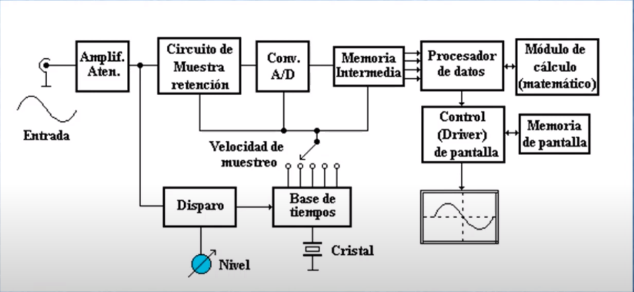
\includegraphics[width=\textwidth]{Imagenes/MarcoTeorico/MathModuleEnOscilDigital.png}}
            \caption{Módulo matemático en Osciloscopio Digital.}
            \label{fig:MathModuleEnOscil}
        \end{figure}
    
    En el modelo de Osciloscopio utilizado en el presente trabajo práctico (TP) es el  
    (\textit{Tektronix TDS 1001}), cuya presentación de pantalla en modo FFT se observa en 
    la Figura~\ref{fig:MathModoEnTek}.   
        \begin{figure}[H]
            \centering
            \frame{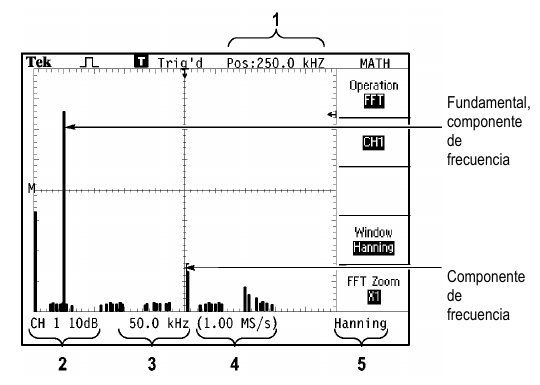
\includegraphics[width=\textwidth]{Imagenes/MarcoTeorico/PresentacionDePantallaFFT.png}}
            \caption{Modo Matemático en Osciloscopio,}
            \label{fig:MathModoEnTek}
        \end{figure}
    Donde se destaca los siguientes puntos 
    \begin{enumerate}
        \item Frecuencia de la linea central de la pantalla.
        \item Escala Vertical en dB/div donde (0 dB = 1 \(V_{RMS}\)).
        \item Escala horizontal en Frec/div.
        \item Velocidad de muestreo. 
        \item Tipo de ventana FFT. 
    \end{enumerate}    

     A continuación, se hace incapie en los tipos de ventanas que se utilizaran en el 
     presente TP como se observa en la Figura~\ref{fig:VentanasTipos} indicando sus 
     ventajas y desventajas.
        \begin{figure}[H]
            \centering
            \begin{subfigure}[H]{0.45\textwidth}
            \frame{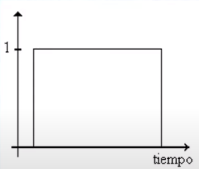
\includegraphics[width=\textwidth]{Imagenes/MarcoTeorico/VentanaRectangular.png}}
            \caption{Ventana Rectangular.}
            \label{fig:VentanaRec}
            \end{subfigure}
            \hfill 
            \begin{subfigure}[H]{0.45\textwidth}
            \frame{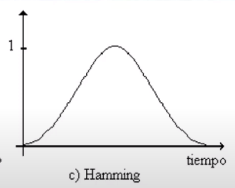
\includegraphics[width=\textwidth]{Imagenes/MarcoTeorico/VentanaHamming.png}} 
            \caption{Ventana Hamming.}
            \label{fig:VentanaHamming}
            \end{subfigure}
            \hfill 
            \begin{subfigure}[H]{0.45\textwidth}
            \frame{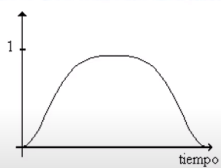
\includegraphics[width=\textwidth]{Imagenes/MarcoTeorico/VentanaFlattop.png}}
            \caption{Ventana flattop.}
            \label{fig:VentanaFlattop}
            \end{subfigure}

            \caption{Tipos de Ventan para FFT.}
            \label{fig:VentanasTipos}
        \end{figure}
    
    La \textbf{ventana rectangular}, Figura~\ref{fig:VentanaRec} posee como ventaja principal su 
    gran utilidad para medir señales con transitorios rápidos. una desventaja notoria de 
    es que, como la misma es una ventana de apertura y cierre abrupto, esto puede 
    generar la aparición a flancos abruptos que no existen realmente en la señal, causando 
    errores en la lectura de la misma.
    
    La \textbf{ventana Hamming}, Figura~\ref{fig:VentanaHamming} se las concidera como una ventana de 
    apertura y cierre suave a diferencia de la rectangular. Esto permite eliminar el problema
    de los flancos abruptos facilitando las mediciones de amplitudes de las componentes 
    espectrales de una señal. Pero como desventaja poseen poca exactitud para realizar 
    mediciones de frecuencias.
    
    Por último la \textbf{ventana flattop}, Figura~\ref{fig:VentanaFlattop} es una solución de compromiso
    entre las dos ventanas previamente mencionadas. 

    \subsubsection*{Uso de Cursores}
        
        Cabe destacar, que también se para realizar las mediciones en los diferentes ensayos
        se utiliza los \textbf{cursores} propios del osciloscopio. Con ellos se puede 
        realizar mediciones en amplitud (dB) o frecuencia tal como se observa en la
        Figura~\ref{fig:CursorTipos}.  
            \begin{figure}[H]
                \centering
                \begin{subfigure}[H]{0.45\textwidth}
                \frame{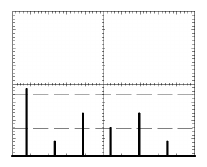
\includegraphics[width=\textwidth]{Imagenes/MarcoTeorico/CursoresEnMagnitud.png}}
                \caption{Cursores en Magnitud.}
                \label{fig:CursorMag}
                \end{subfigure}
                \hfill 
                \begin{subfigure}[H]{0.45\textwidth}
                \frame{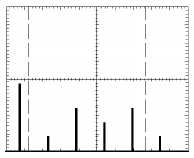
\includegraphics[width=\textwidth]{Imagenes/MarcoTeorico/CursoresEnFrecuencia.png}}
                \caption{Cursores en Frecuencia.}
                \label{fig:CursorFrec}
                \end{subfigure}
                \caption{Tipos de cursores del Osciloscopio Digital.}
                \label{fig:CursorTipos}
            \end{figure}

        Se debe tener presente que cuandos e realiza mediciones de magnitudes de las 
        componentes en frecuencia con el osciloscopio, dichas magnitudes dada en 
        decibleles esta referenciada a valor de \(V_{RMS}\) y no de amplitud pico de la señal.
                
    

    



